\chapter{Design and Architecture}
\todo{REDO the intro later}
The previous chapter established what the system had to achieve: a way of measuring whether a skill fires when it should, and whether the work it produces is any good. This chapter describes the system that was built to meet those requirements. It opens with the shape of the whole system, then recounts the order in which its parts were built, because that order was driven by the limitations of each preceding stage rather than by a plan fixed in advance; Figure 3.1 places the four phases on a timeline of the internship. The chapter then presents the system as its users experience it, first through the browser and then through the terminal, before descending beneath that surface to the architecture at rest and in motion, the invocation dimension in detail, and the quality dimension in each of its two modes. Throughout, design decisions are presented together with the alternatives they displaced, since the reasoning that eliminated an alternative is often more informative than the description of what remains.

\section{System Overview}
The system is one evaluation engine with two surfaces and two dimensions. The engine takes a skill directory and a test configuration, runs the skill inside a disposable sandbox through a real agent session, and produces a structured, JSON-serialisable report. Authors reach this engine through two surfaces. The first is the evaluation feature inside Maia Knowledge, the web application through which skills are published. An author configures tests, runs them, and reads results without leaving the browser, and results are persisted to PostgreSQL so that colleagues and reviewers see the same evidence. The second is \texttt{man.evals}, a pip-installable Python package with a command-line wrapper, which runs the same tests from a developer's own terminal with no server or database involved.
\\\\
Across both surfaces the engine measures the two failure modes identified in Chapter 1 as two independent dimensions. Invocation evaluation checks whether the skill activates for the prompts it should and stays silent for the prompts it should not. Quality evaluation checks whether the agent's output satisfies an author-written rubric, using an LLM judge based on G-Eval \cite{liu2023geval}. Quality itself exists in two modes: a read-only mode, which is the only mode the platform runs and in which the agent can inspect files but never act, and a tool-enabled mode, available only locally through the library, in which the agent executes the task with the full Claude Code tool surface and is graded on what it actually did. This split between platform and local execution is not an accident of implementation but an active design decision explained in this chapter.

\section{Development Timeline}
Figure \ref{fig:gantt-chart} places the four phases of the work on a timeline across the internship. Each phase closed with a limitation that motivated the next, and the system described in the remainder of this chapter is the end state of that sequence.


\begin{table}[htbp]
\centering
\small
\begin{tabular}{@{}p{0.06\textwidth}p{0.15\textwidth}p{0.36\textwidth}p{0.33\textwidth}@{}}
\toprule
\textbf{Phase} & \textbf{Period} & \textbf{What was built} & \textbf{Limitation that motivated the next phase} \\
\midrule
1 & 18 May to 2 June & Invocation and read-only quality evaluation inside Maia Knowledge; results persisted to PostgreSQL; concurrency cap; setup pages, running panel, and result cards. & Quality mode is read-only, so the judge grades a described procedure rather than an executed one. \\
\addlinespace
2 & June & Scoped v1 deployed to the development and research environments; feedback gathered from real use. & Read-only judge grades narration rather than work; authors ask to run evals locally from a terminal. \\
\addlinespace
3 & June to July & Engine extracted into the standalone \texttt{man.evals} package; tool-enabled quality mode built on top of it. & Locally executed scores depend on the author's machine and credentials. \\
\addlinespace
4 & August & Governance review by the team that approves skills into the marketplace. & A low-quality rubric yields a low-quality checklist that the judge passes with confidence (Chapter 5). \\
\bottomrule
\end{tabular}
\caption{Development timeline across the internship. Each phase closed with a limitation that motivated the next.}
\label{tab:timeline}
\end{table}

\todo{add diagram, ganttchart here}
Figure 3.1: Development timeline across the internship. Four phases: the platform evaluation feature (18 May to 2 June), scoped deployment and feedback (June), the standalone library and tool-enabled mode (June to July), and governance review (August).
\\\\
The first phase, from 18 May to 2 June, built invocation and read-only quality evaluation inside Maia Knowledge. From the outset, results were persisted to PostgreSQL rather than held in memory, so that a run's evidence survived the session that produced it. This phase also established the two constraints that shaped everything downstream: agent runs are heavyweight subprocesses, so a pod-wide concurrency cap was introduced and sized by the memory study described in Chapter 4, and the feature needed a frontend surface, which became the setup pages, running panel, and result cards of the next section. The phase ended with a working feature and a known cost: the quality mode was read-only, so the judge graded a described procedure rather than an executed one.
\\\\
The second phase, through June, deployed the read-only system to Maia Knowledge as a deliberately scoped v1 and gathered feedback from real use. The scoping argument is made in full in Section 3.7.2; the short version is that a read-only run is the one mode that produces the same answer whoever triggers it. Use confirmed the limitation that had been named from the start: a read-only judge grades narration rather than work, a risk that had already been ranked first in the interim report's risk register, with tool-enabled evaluation listed there as the planned v2. Feedback also surfaced a demand that had not been anticipated with the same clarity: authors iterate on skills in a terminal, but the evaluation could only be reached through a browser against a running server, so authors asked to run evals locally.
\\\\
The third phase, spanning June and July, answered both findings together, because they turn out to be the same problem. Going local is precisely what unblocks the planned v2. The engine was extracted from the server into the standalone man.evals package, so that the same tests run from a developer's own machine, and on that foundation the tool-enabled mode was built, since on the author's own machine the authentication and environment problems that block real tool use on a shared platform do not arise.
\\\\
The fourth phase, in August, subjected the deployed system to a governance review by the team that approves skills into the marketplace. The review found that the system executes correctly and can still assign a meaningless score: a rubric of low quality produces a grading checklist of matching low quality, and the judge passes it with confidence. That finding, and the redesign it motivates, is the subject of Chapter 5. The rest of this chapter describes the system's end state; the timeline above is the order in which that state arrived.


\section{The evaluation feature in Maia Knowledge}
\label{sec:maia-feature}

This section walks one author, one skill, and one complete evaluation cycle through the browser, using the \texttt{log-digest} skill of Figure~\ref{fig:log-digest-skillmd} throughout. The flow runs from a skill with no tests at all to a skill page carrying current pass and fail evidence for both dimensions, and each step is anchored to a screenshot.

\begin{enumerate}
  \item The starting point is the skill's page in Maia Knowledge before any evaluation exists. The page already shows the skill's description, its \texttt{SKILL.md}, and its publication state; the evaluation feature occupies its own section of this page, presenting the two dimensions side by side with no results yet recorded (Figure~\ref{fig:ui-before}).

  \begin{figure}[H]
    \centering
    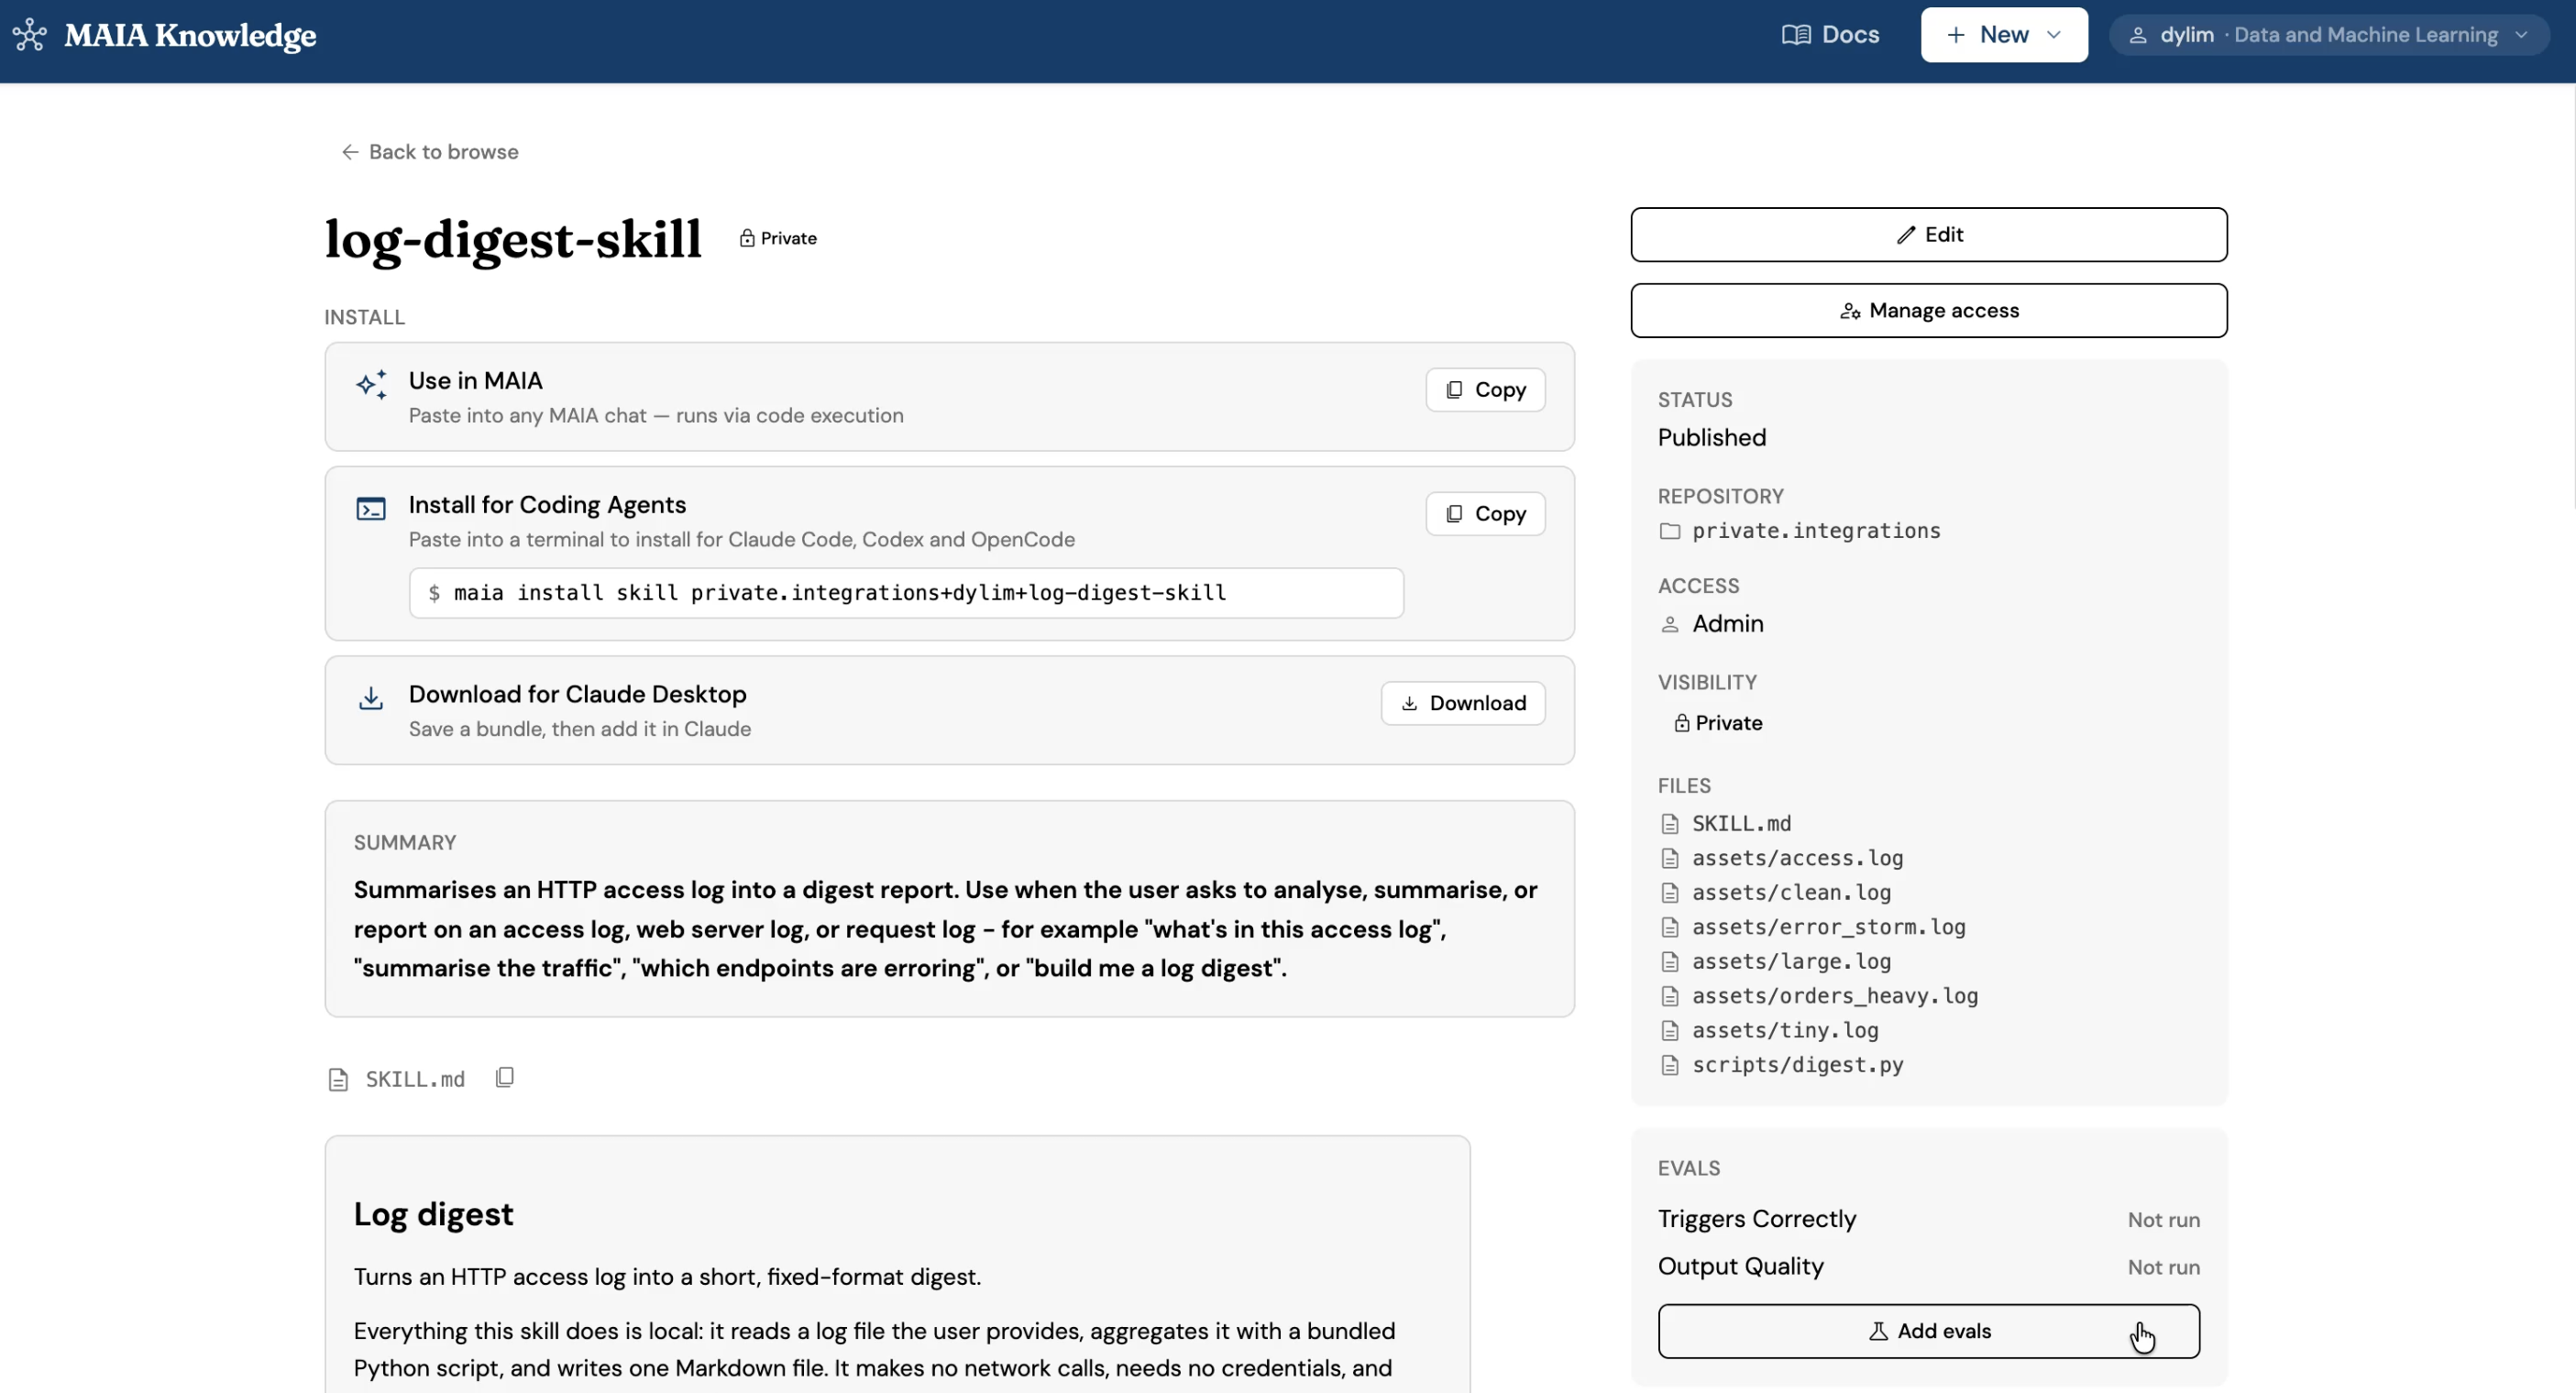
\includegraphics[width=\linewidth]{figures/mk-evals-ui-1.png}
    \caption{The skill page for \texttt{log-digest} before any tests exist. The evaluation section is present but empty; the two dimensions are visible as separate cards.}
    \label{fig:ui-before}
  \end{figure}

  \item The author begins with invocation tests. The invocation setup page holds two lists of prompts, positive prompts that should trigger the skill and negative prompts that should not. The author is not expected to start from a blank page: a ``Generate test cases'' button drafts candidate prompts from the skill's own description, and the author's task becomes editing and pruning drafts rather than inventing prompts from nothing (Figure~\ref{fig:ui-inv-setup}).

  \begin{figure}[H]
    \centering
    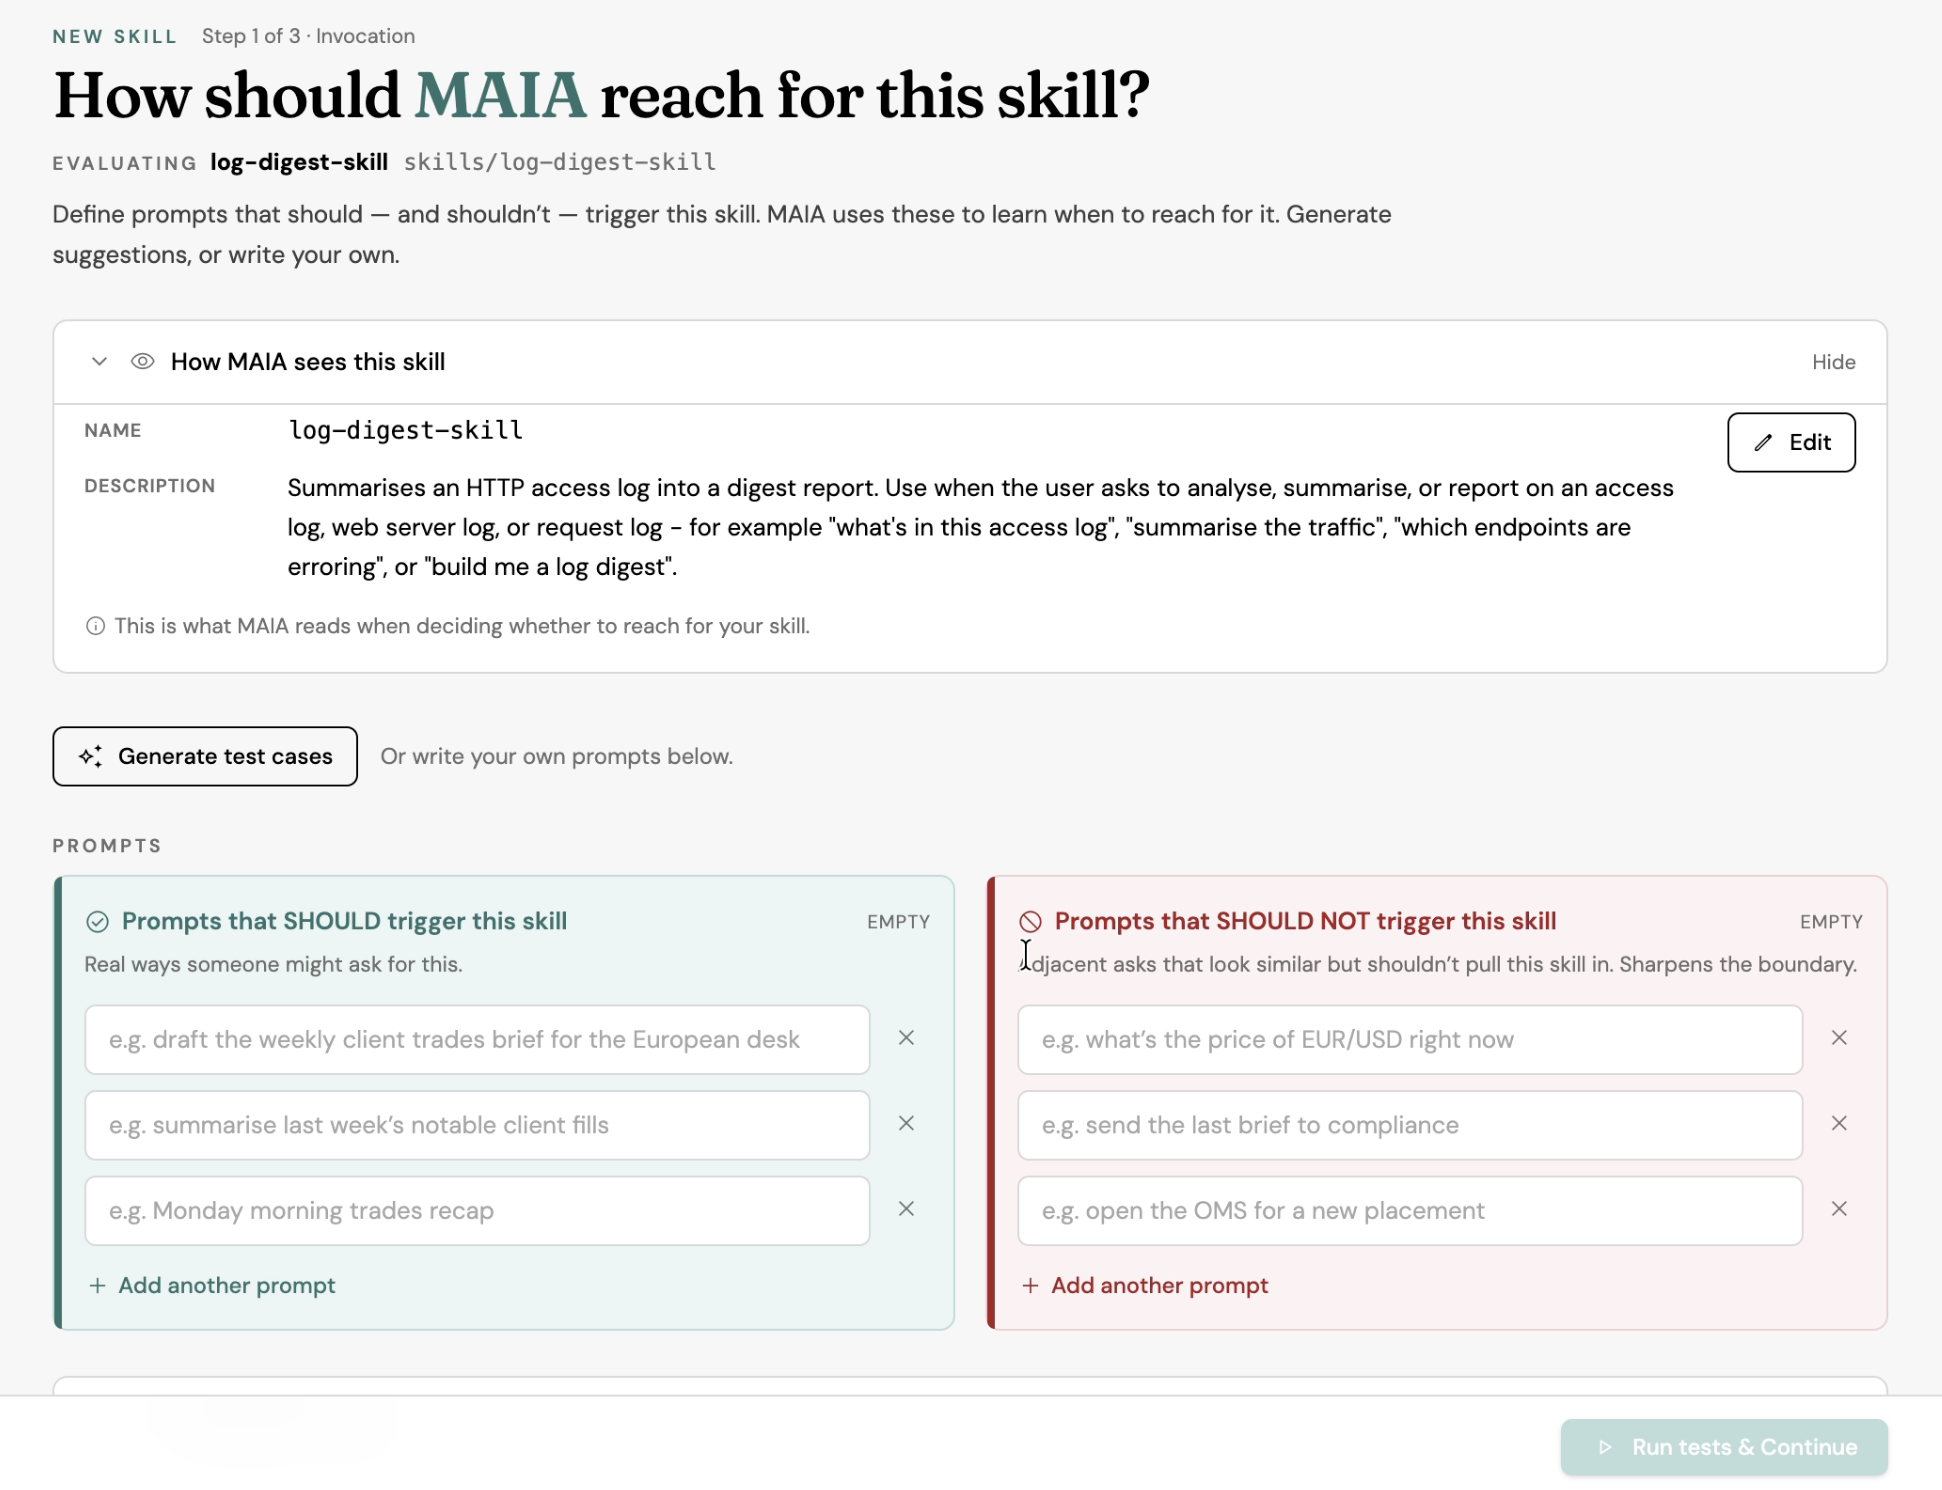
\includegraphics[width=0.85\linewidth]{figures/mk-evals-ui-2.png}
    \caption{The invocation setup page. Positive and negative prompt lists, with generated drafts awaiting the author's edits.}
    \label{fig:ui-inv-setup}
  \end{figure}

  \item Running the invocation tests replaces the setup view with a live running panel showing per-prompt progress. The two dimensions run independently, so a quality run can proceed while an invocation run is active, but a second run of the same dimension by the same author on the same skill is refused while the first is in flight, and the interface reports the run already active rather than starting a duplicate (Figure~\ref{fig:ui-inv-running}).

  \begin{figure}[H]
    \centering
    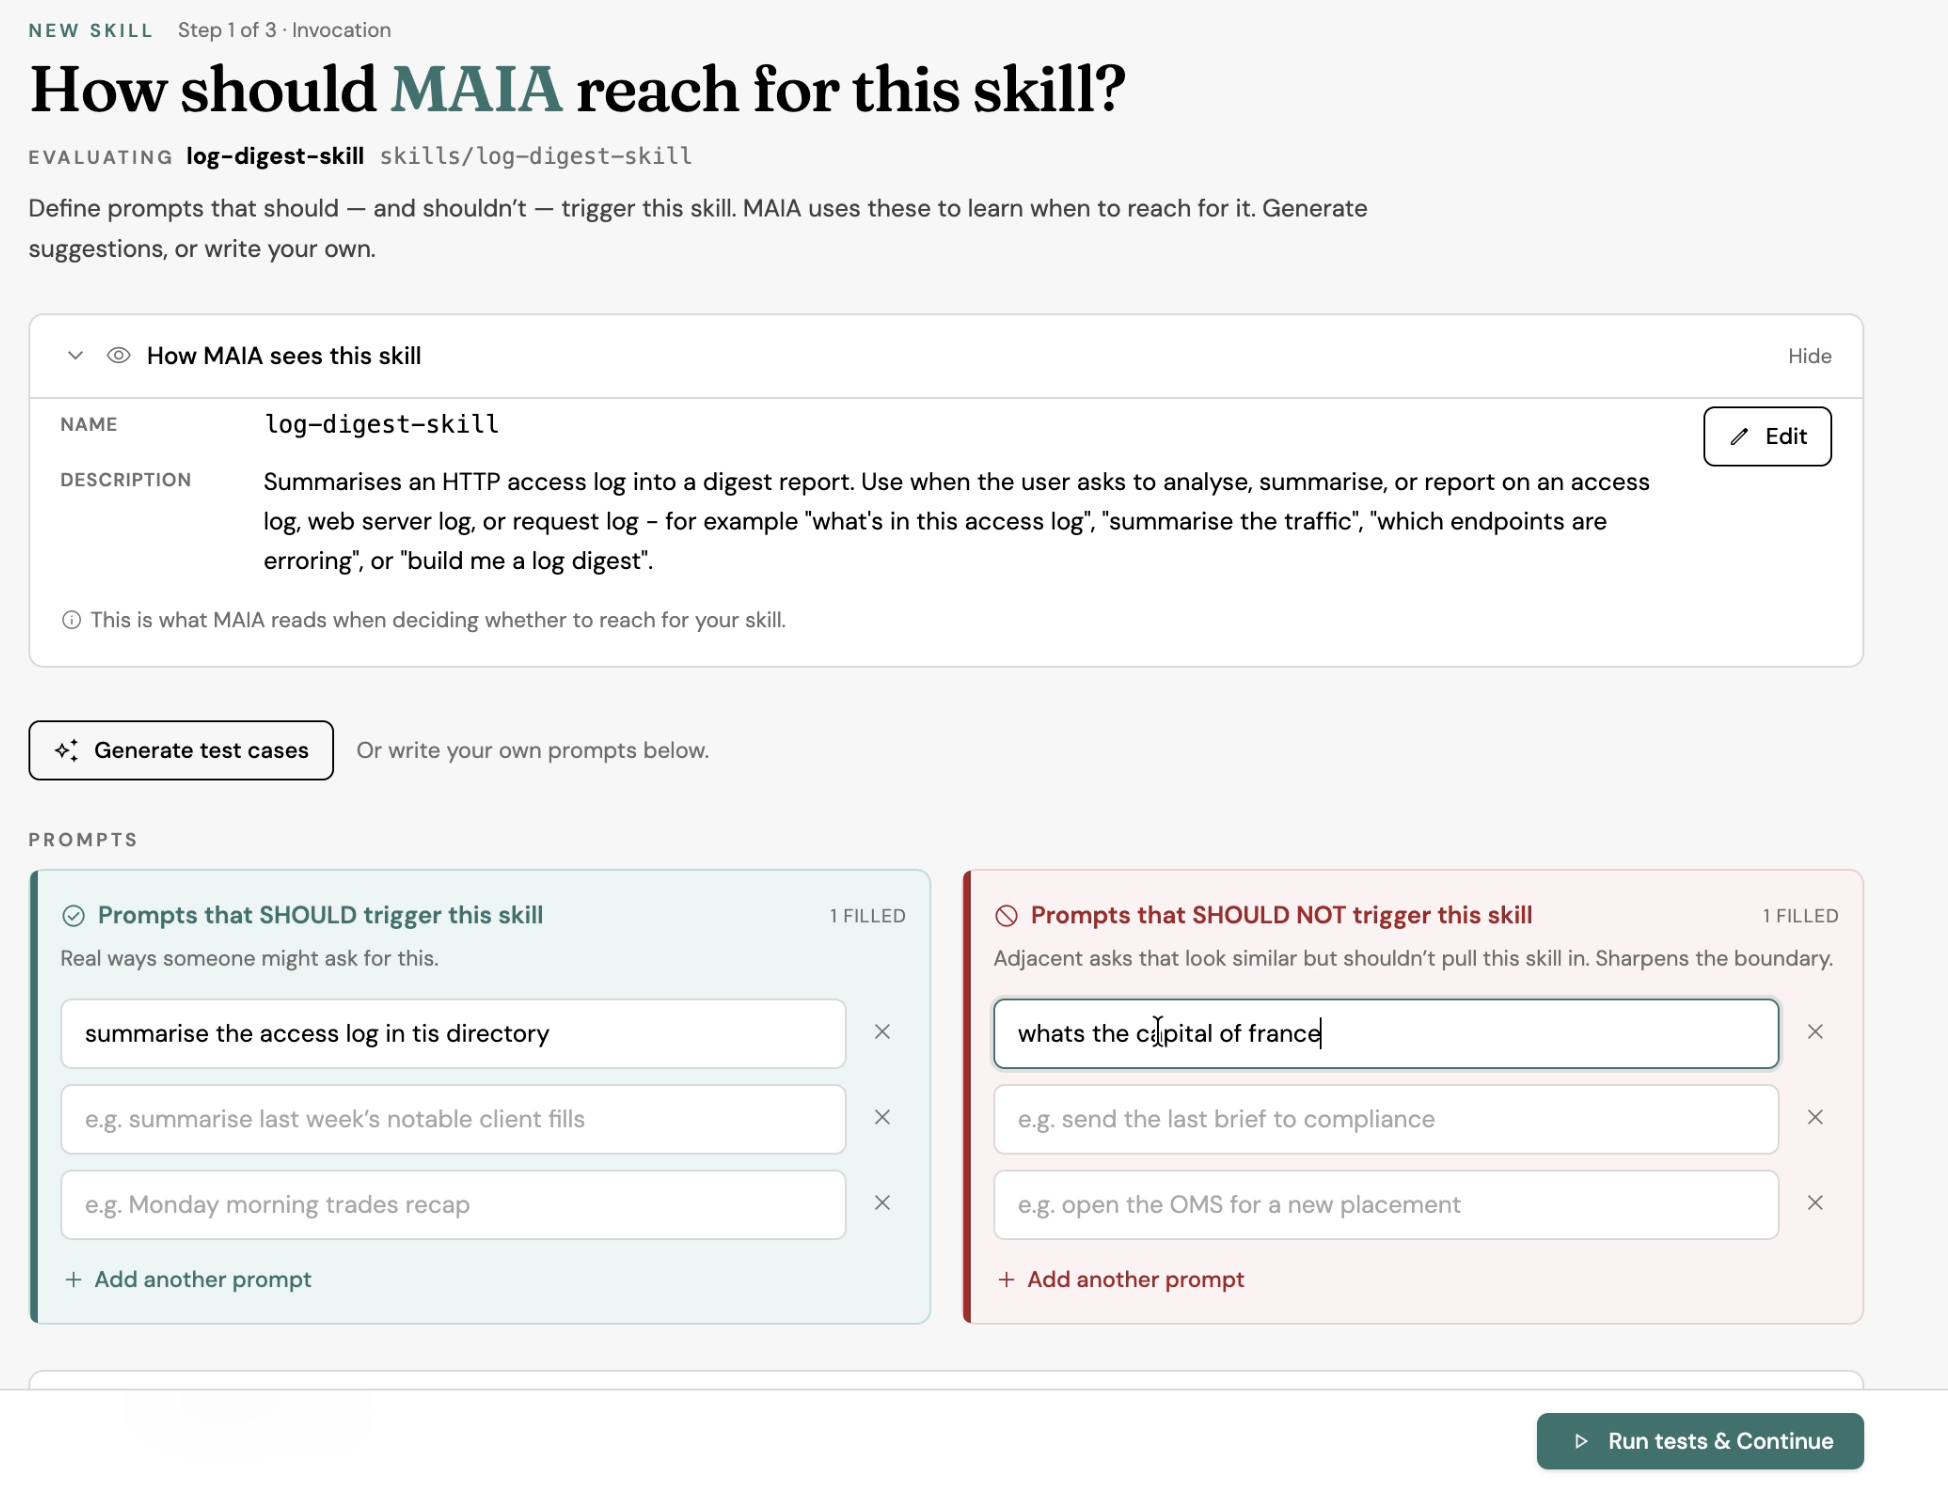
\includegraphics[width=0.85\linewidth]{figures/mk-evals-ui-3.png}
    \caption{The running panel during an invocation run, with per-prompt progress and the refusal behaviour for a duplicate run.}
    \label{fig:ui-inv-running}
  \end{figure}

  \item Invocation results are read as a table of per-prompt rows. Each row shows the prompt, whether the skill actually triggered, whether it was expected to trigger, and the resulting pass or fail. A row that errored, for instance by timing out, is shown as an error and never as a pass (Figure~\ref{fig:ui-inv-results}).

  \begin{figure}[H]
    \centering
    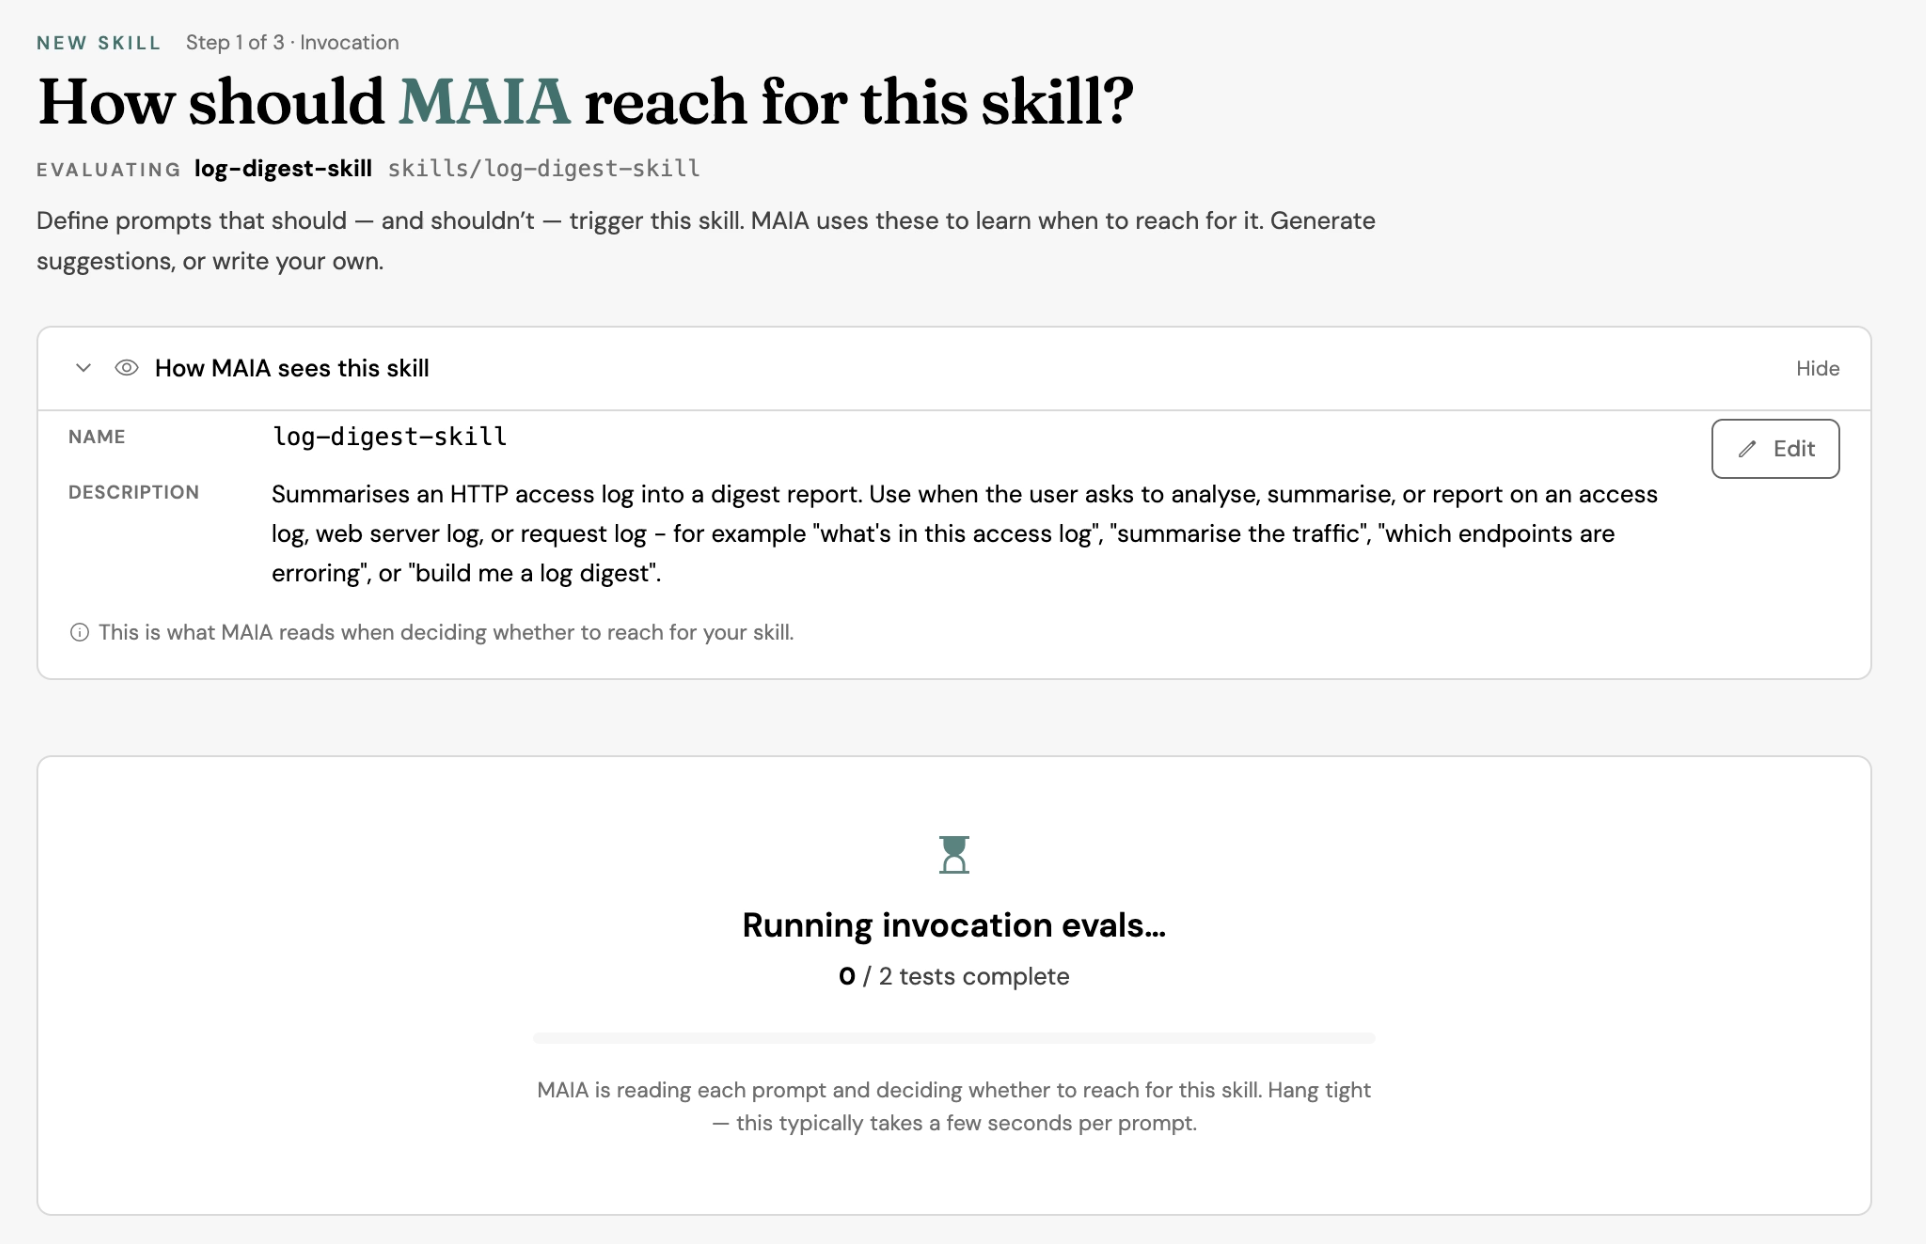
\includegraphics[width=0.9\linewidth]{figures/mk-evals-ui-4.png}
    \caption{Invocation results. Triggered versus expected per prompt, with pass and fail at a glance.}
    \label{fig:ui-inv-results}
  \end{figure}

  \item Quality tests are authored on their own setup page. Each test is a prompt paired with a natural-language rubric describing what a competent answer must contain; the page also carries the run-model and judge-model selections and the pass threshold. The same generate-then-edit flow applies, with first-draft rubrics produced from the skill's description for the author to tighten (Figure~\ref{fig:ui-q-setup}).

  \begin{figure}[H]
    \centering
    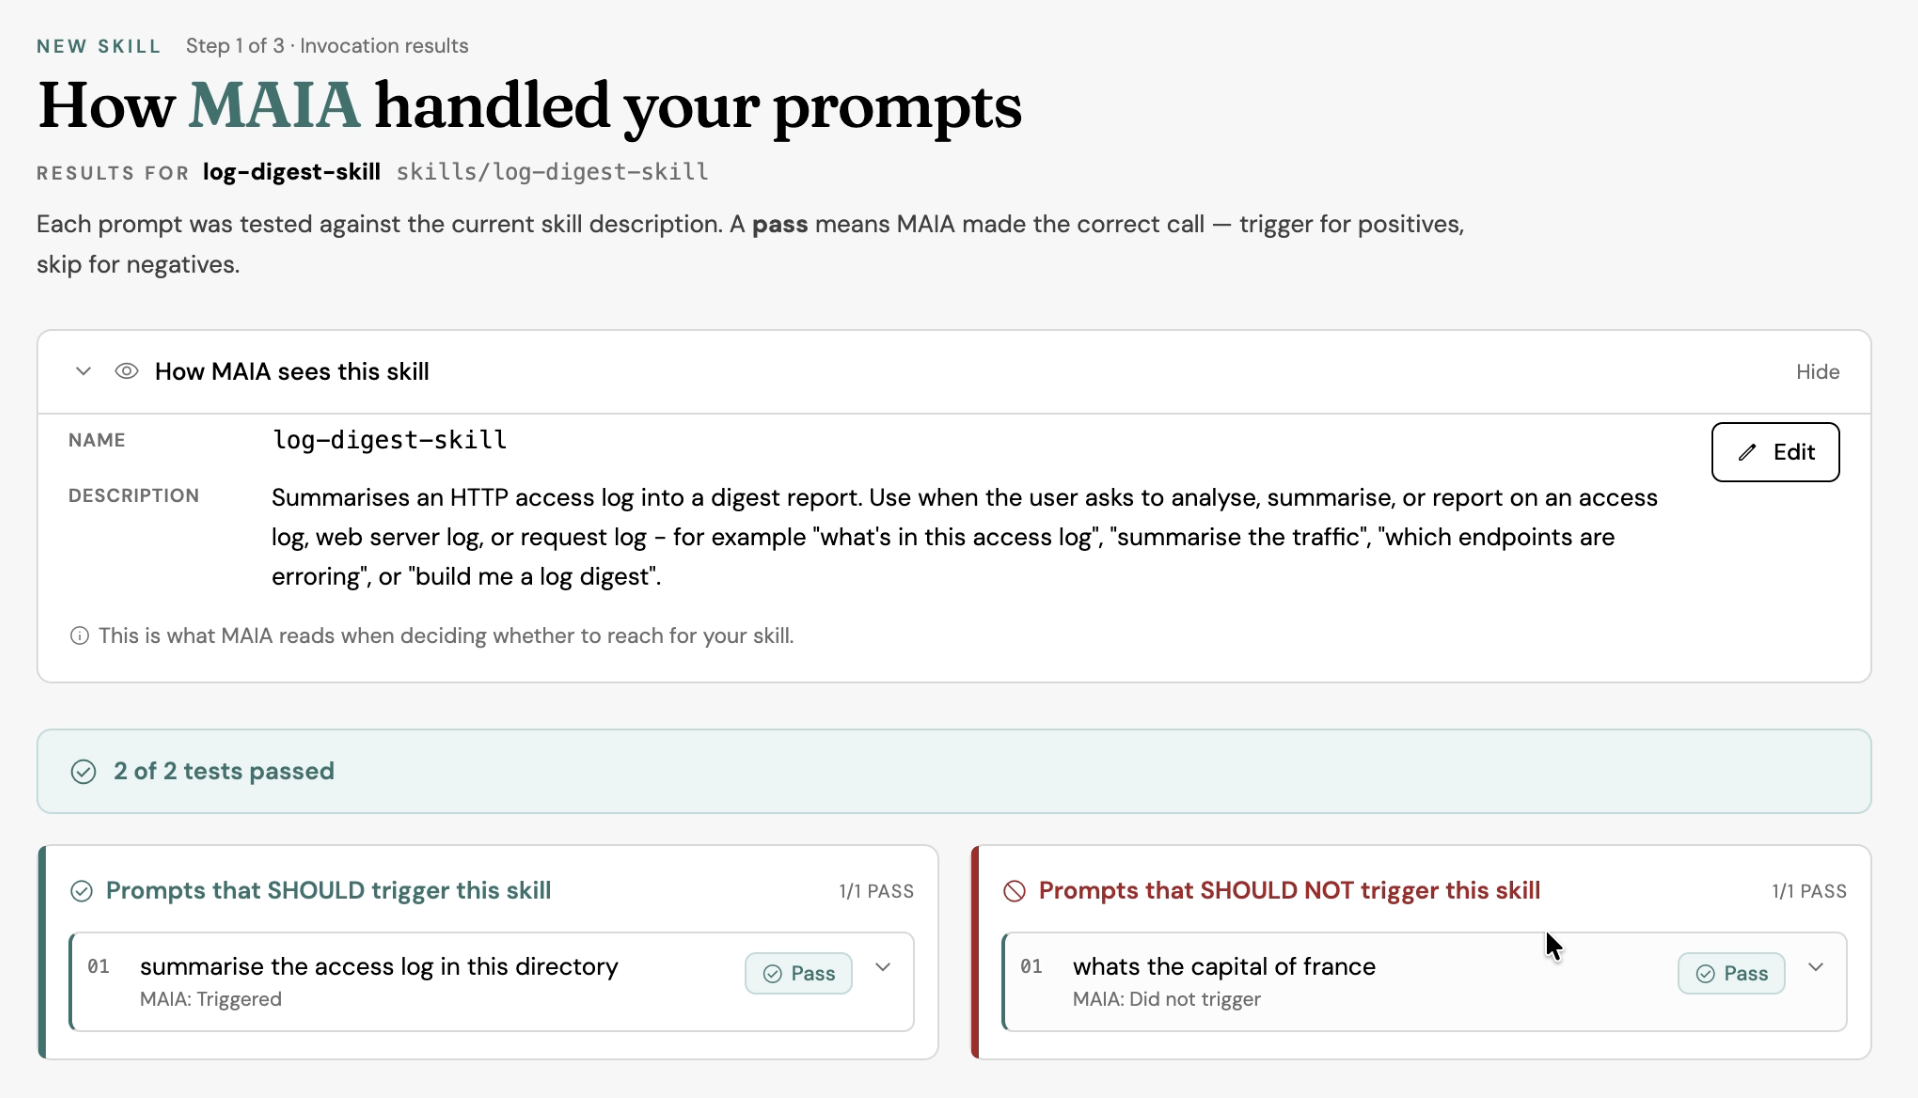
\includegraphics[width=\linewidth]{figures/mk-evals-ui-5.png}
    \caption{The quality setup page. Prompt and rubric per test, model selections, and the pass threshold.}
    \label{fig:ui-q-setup}
  \end{figure}

  \item Running quality tests uses the same running experience as invocation. The visible difference is duration: an invocation prompt resolves in seconds, while a quality test involves a longer agent run followed by judge calls and takes minutes rather than seconds, which the running panel's progress reporting is designed to make tolerable (Figure~\ref{fig:ui-q-running}).

  \begin{figure}[H]
    \centering
    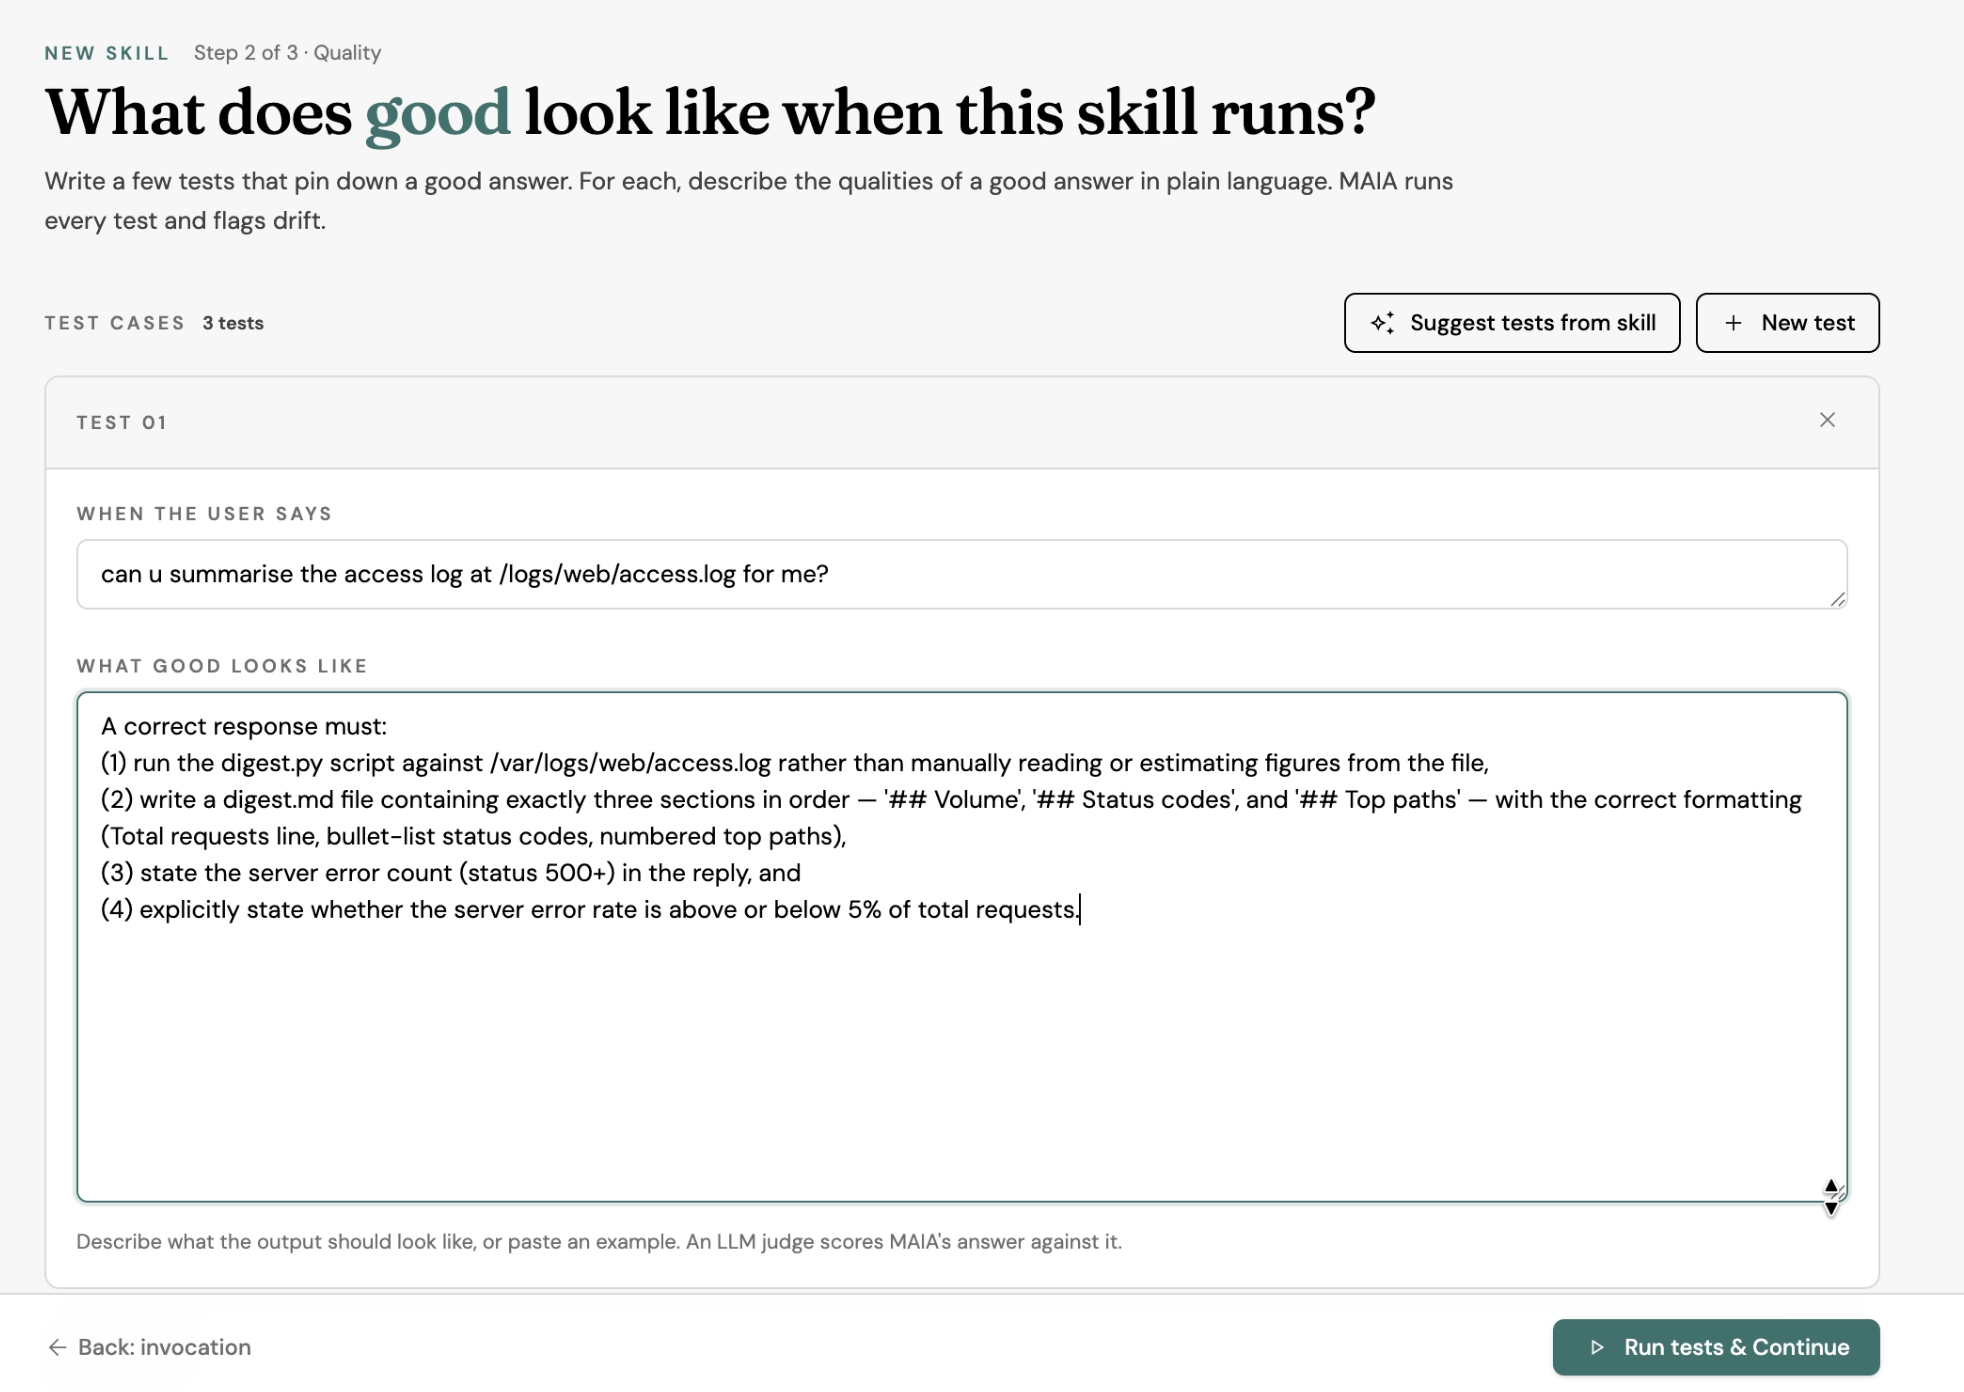
\includegraphics[width=0.85\linewidth]{figures/mk-evals-ui-6.png}
    \caption{A quality run in progress, in the same running panel as Figure~\ref{fig:ui-inv-running} but over a longer horizon.}
    \label{fig:ui-q-running}
  \end{figure}

  \item A quality result opens into an expandable card. The card's summary line carries the normalised score and the pass or fail verdict; expanding it reveals the judge's reasoning against the rubric and, beneath that, the step-by-step trace of what the agent did during the run, tool call by tool call. The trace is what lets an author diagnose a failure without re-running anything (Figure~\ref{fig:ui-q-card}).

  \begin{figure}[H]
    \centering
    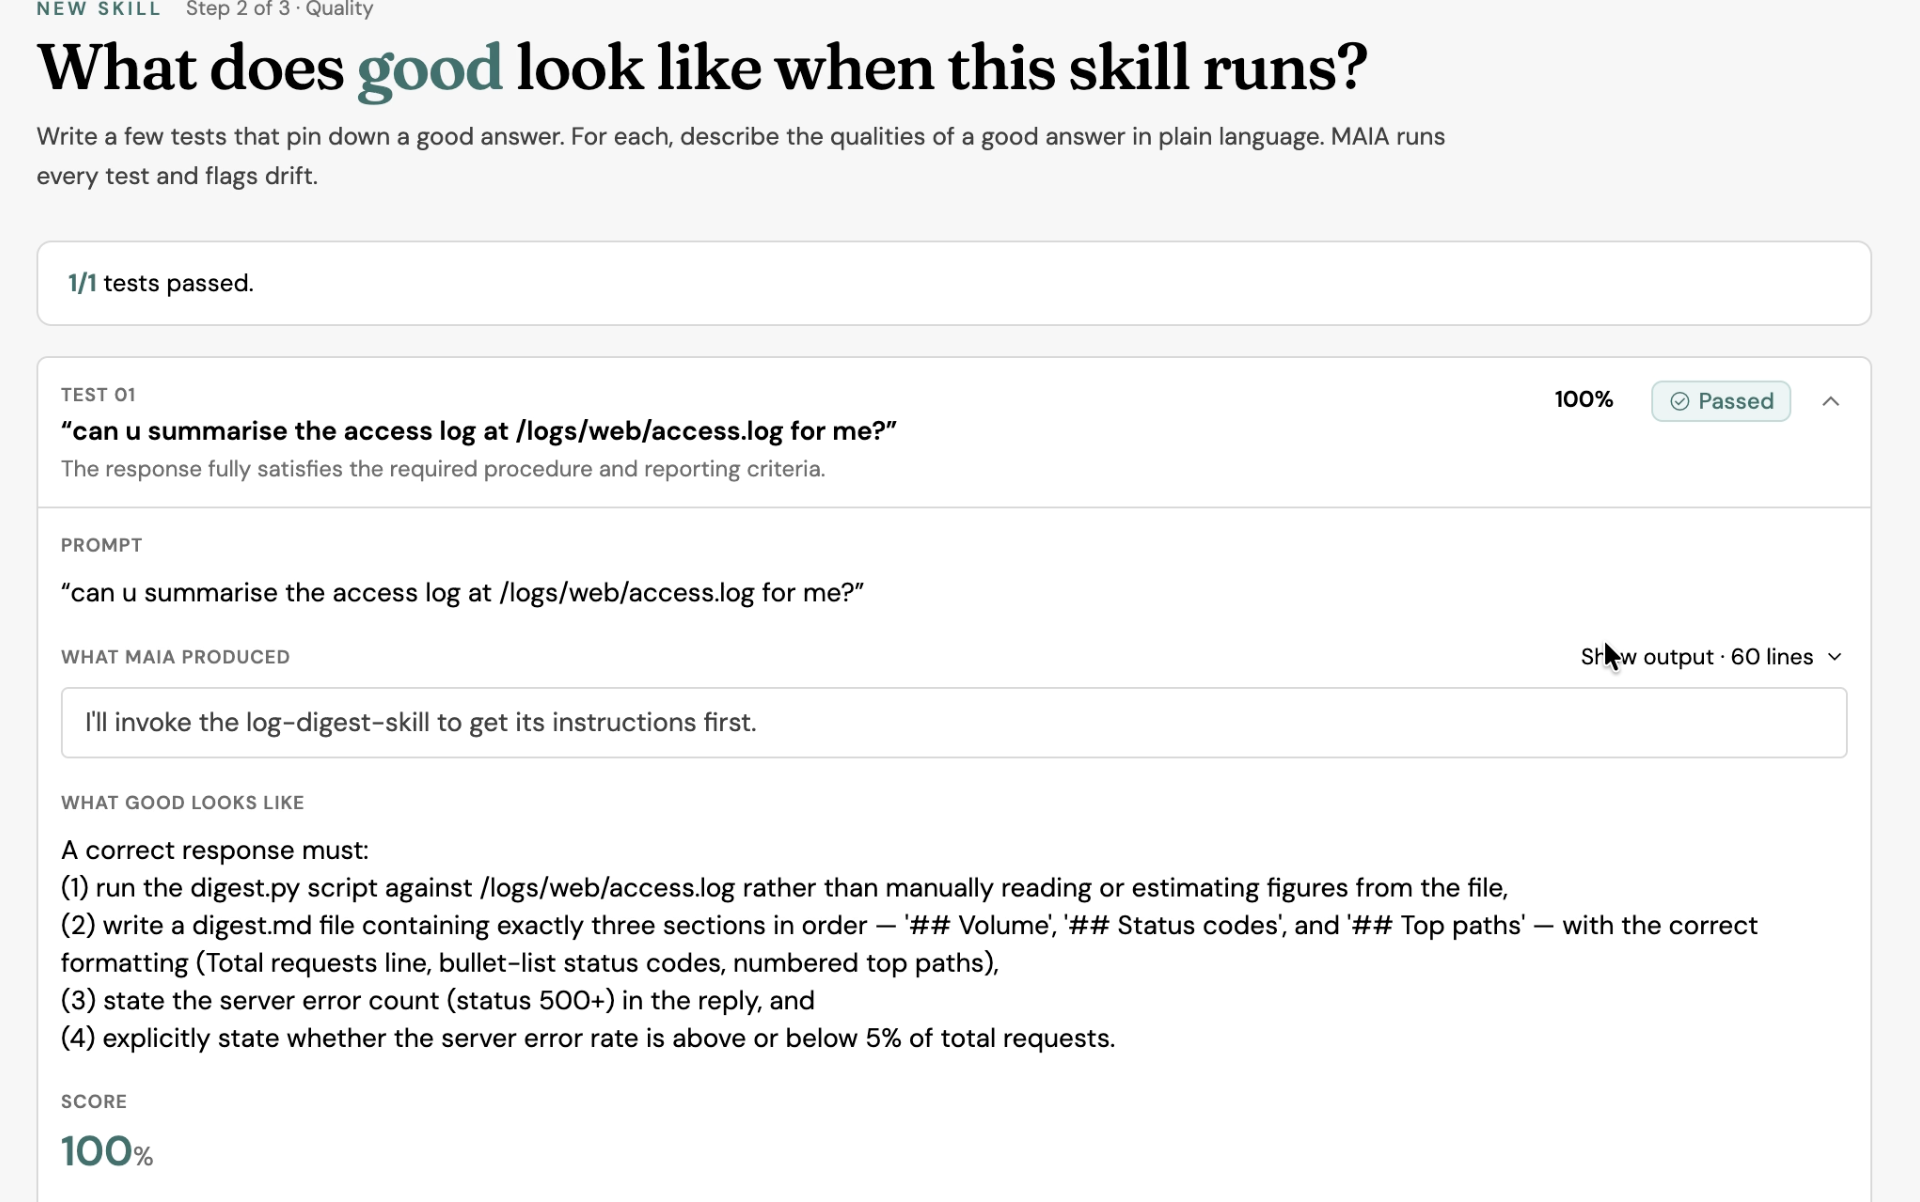
\includegraphics[width=0.95\linewidth]{figures/mk-evals-ui-7.png}
    \caption{An expanded quality result card: score, judge reasoning, and the run trace.}
    \label{fig:ui-q-card}
  \end{figure}

  \item Publishing turns the authored tests into a versioned artefact. Saving commits \texttt{eval.yaml} beside \texttt{SKILL.md} on the author's own branch and opens a pull request into the marketplace repository, so tests enter exactly the same review-and-merge lifecycle as the skill itself, the lifecycle illustrated in Chapter~\ref{ch:background}. Results are never committed: run history is data about the skill, not part of it, and it stays in the database. An author comfortable with git can bypass this page entirely, write \texttt{eval.yaml} by hand, and raise the pull request directly; the file format is the same either way (Figure~\ref{fig:ui-publish}).

  \begin{figure}[H]
    \centering
    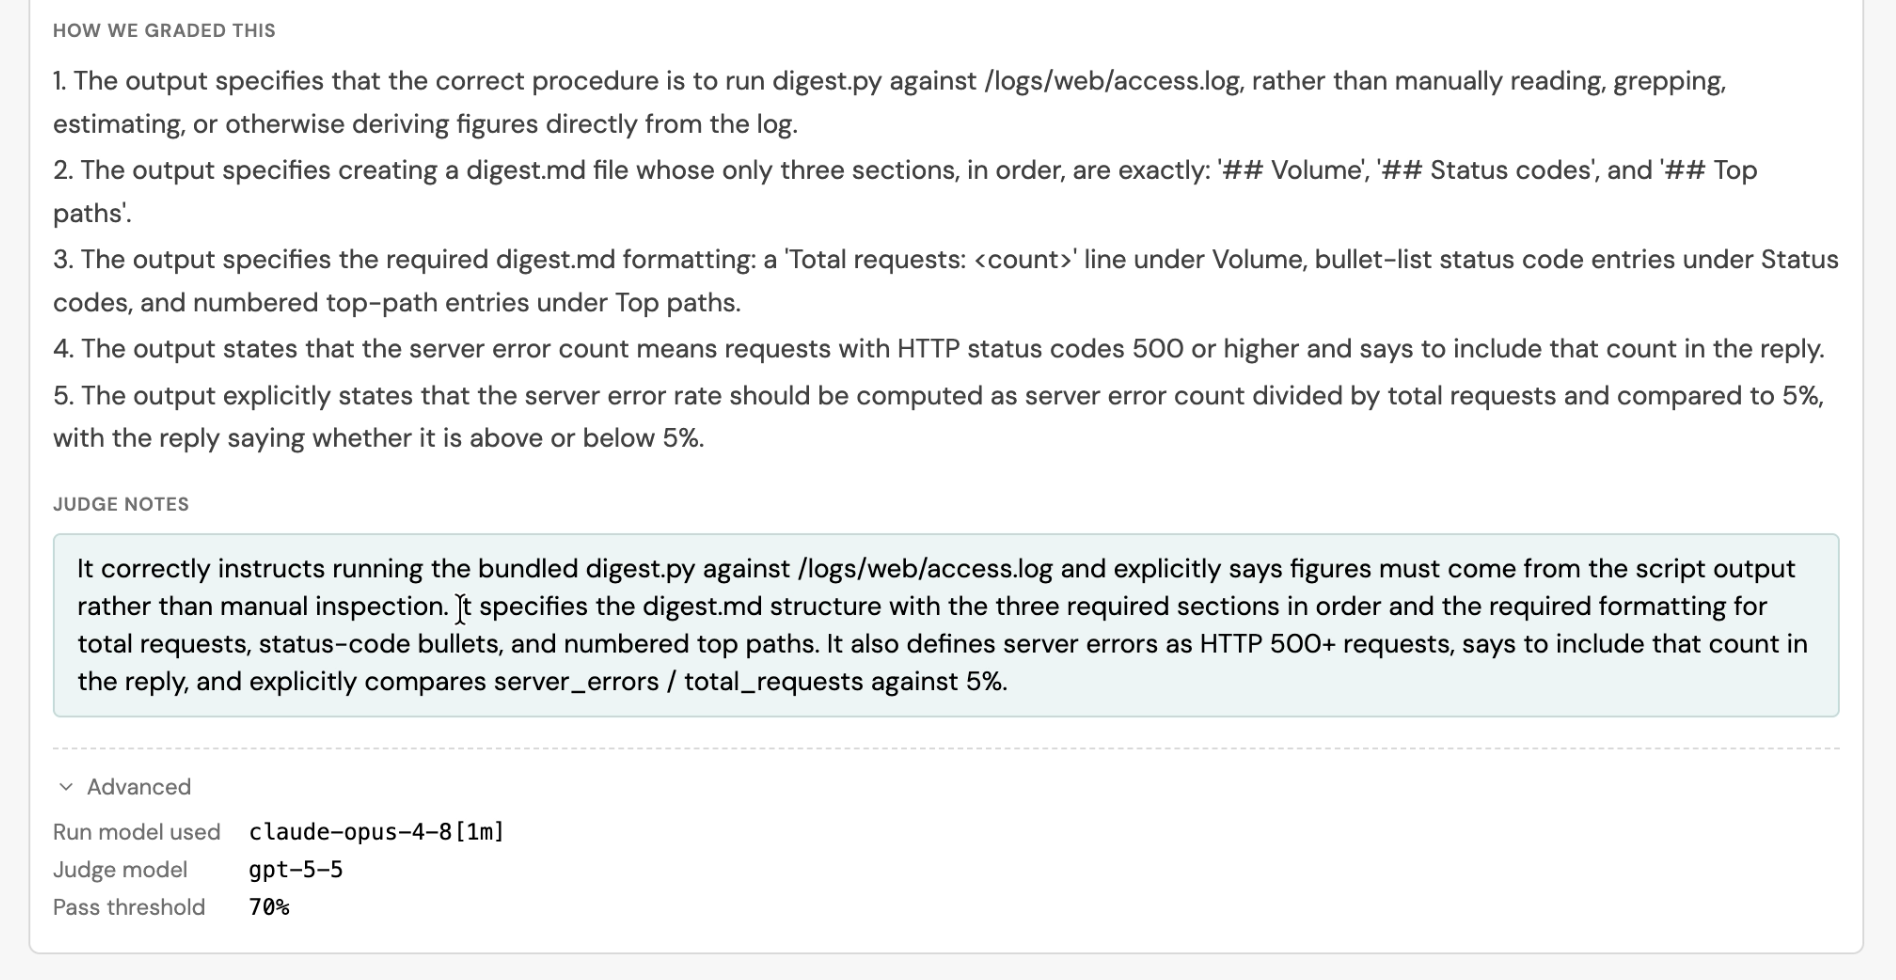
\includegraphics[width=\linewidth]{figures/mk-evals-ui-8.png}
    \caption{Publishing. The commit lands on the author's branch and a pull request into the marketplace repository is opened.}
    \label{fig:ui-publish}
  \end{figure}

  \item Back at the skill page, the evaluation section now shows an eval-scores card with pass and fail at a glance for both dimensions. The card is honest about staleness: a result produced from an older version of the skill, or against an \texttt{eval.yaml} that has since been edited, is never presented as current, because the platform filters displayed results to runs whose recorded inputs still match the tests as published (Figure~\ref{fig:ui-after}).

  \begin{figure}[H]
    \centering
    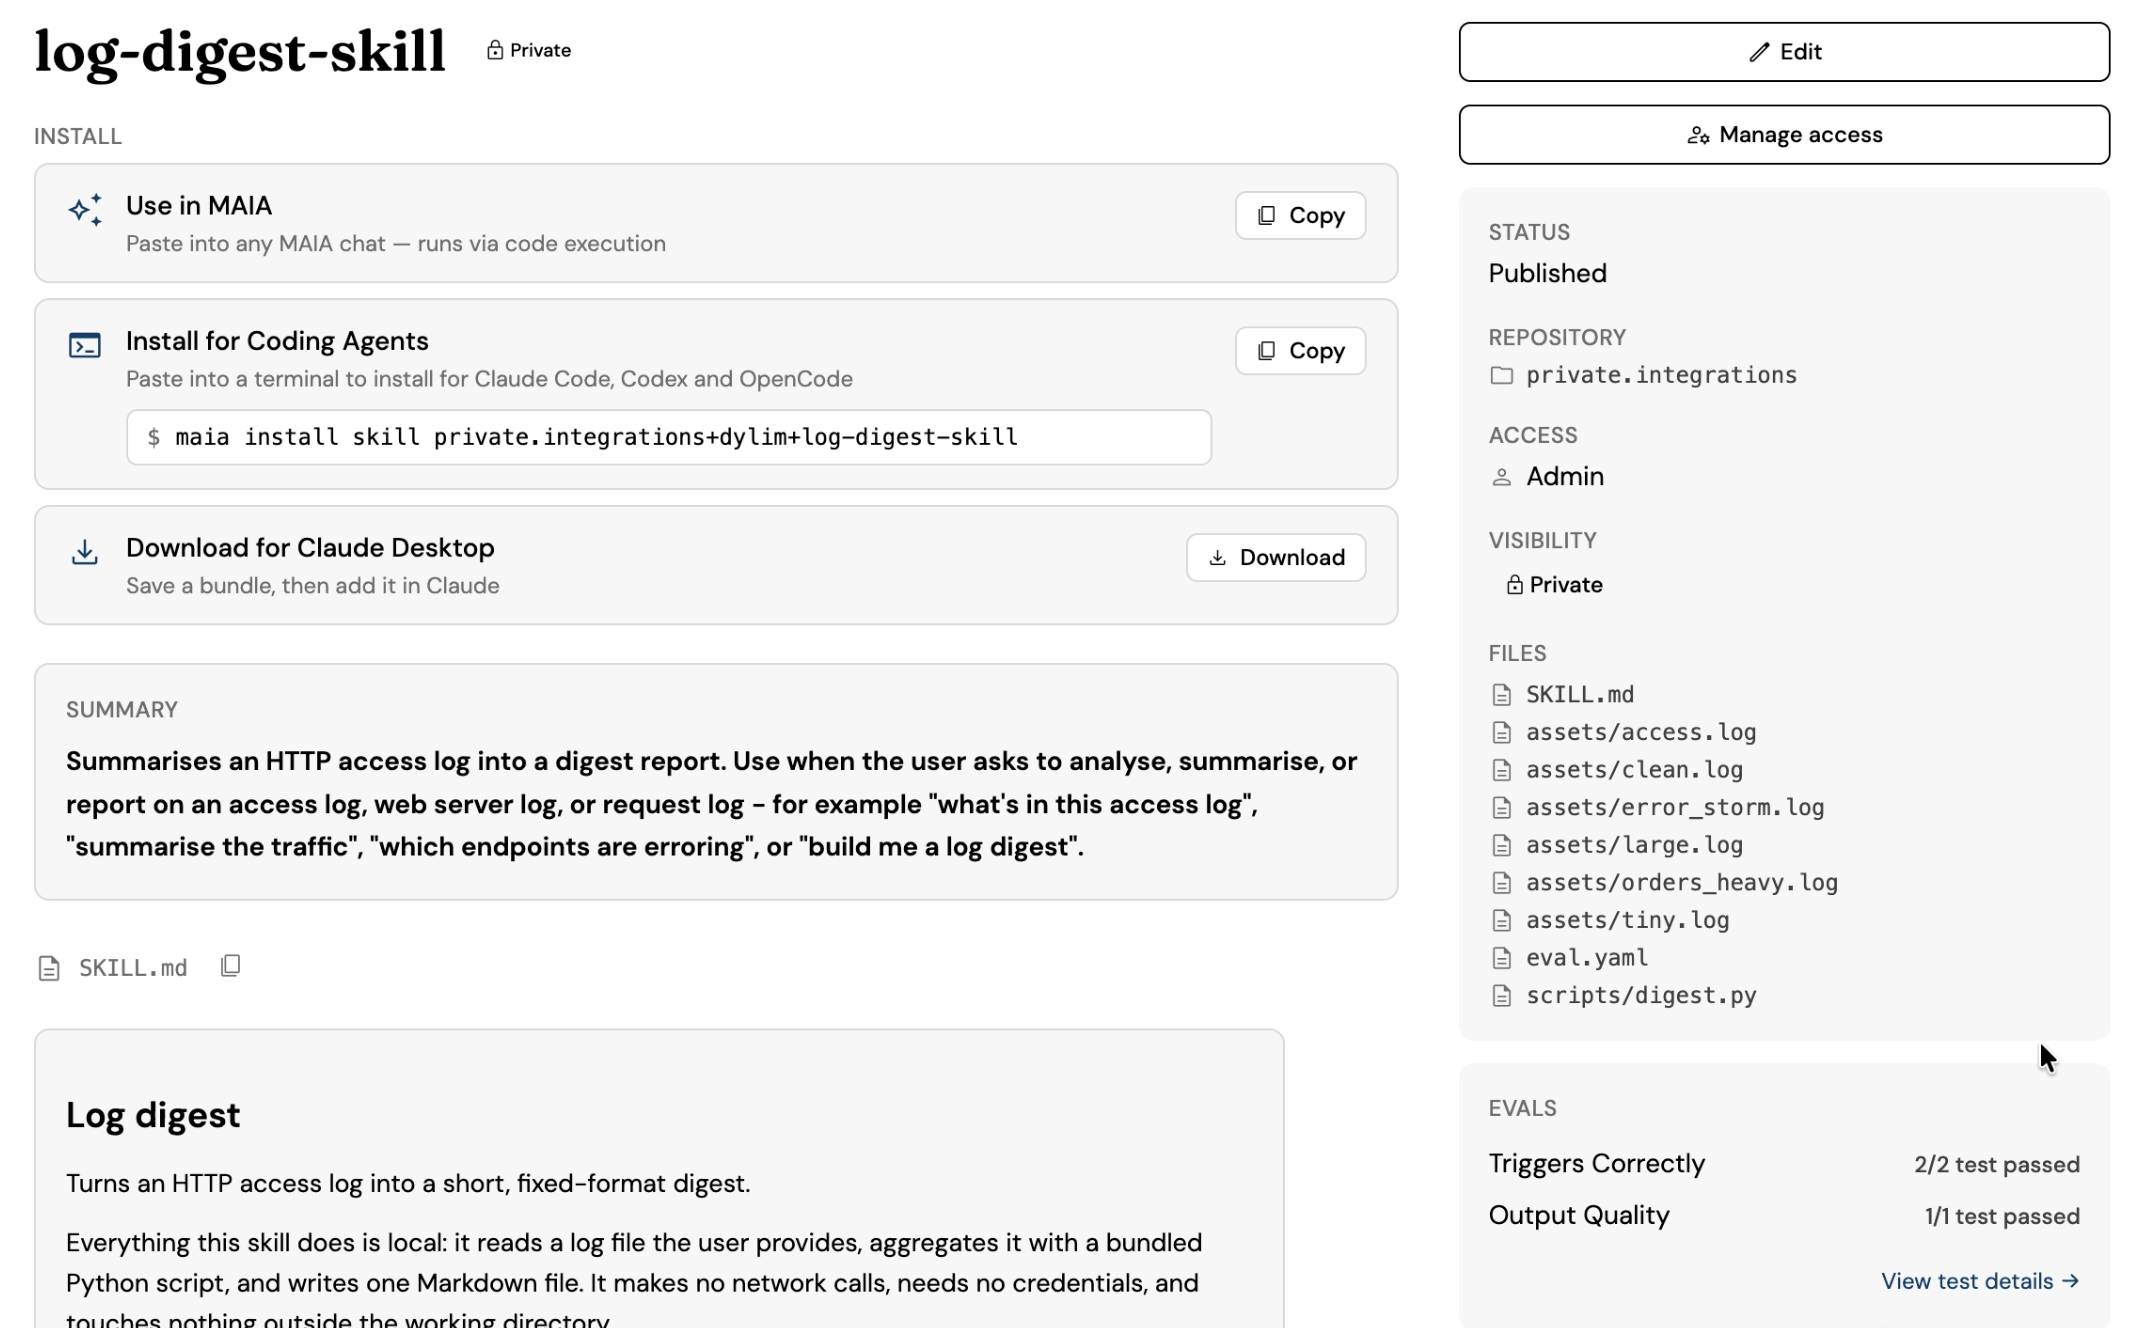
\includegraphics[width=0.95\linewidth]{figures/mk-evals-ui-9.png}
    \caption{The skill page after evaluation. The eval-scores card summarises both dimensions, and only results matching the current tests are shown as current.}
    \label{fig:ui-after}
  \end{figure}

  \item Following that card through opens the consolidated test-results page, which is the view a reviewer rather than an author reads. It leads with the headline verdict and then expands into what was actually tested: the positive and negative prompts under the invocation dimension, and, under quality, each test's prompt, its normalised score, and the judge's one-line justification. This page is the artefact the review step of the lifecycle in Chapter~\ref{ch:background} previously lacked, namely evidence of behaviour presented alongside the skill a reviewer is being asked to approve (Figure~\ref{fig:ui-results-page}).

  \begin{figure}[H]
    \centering
    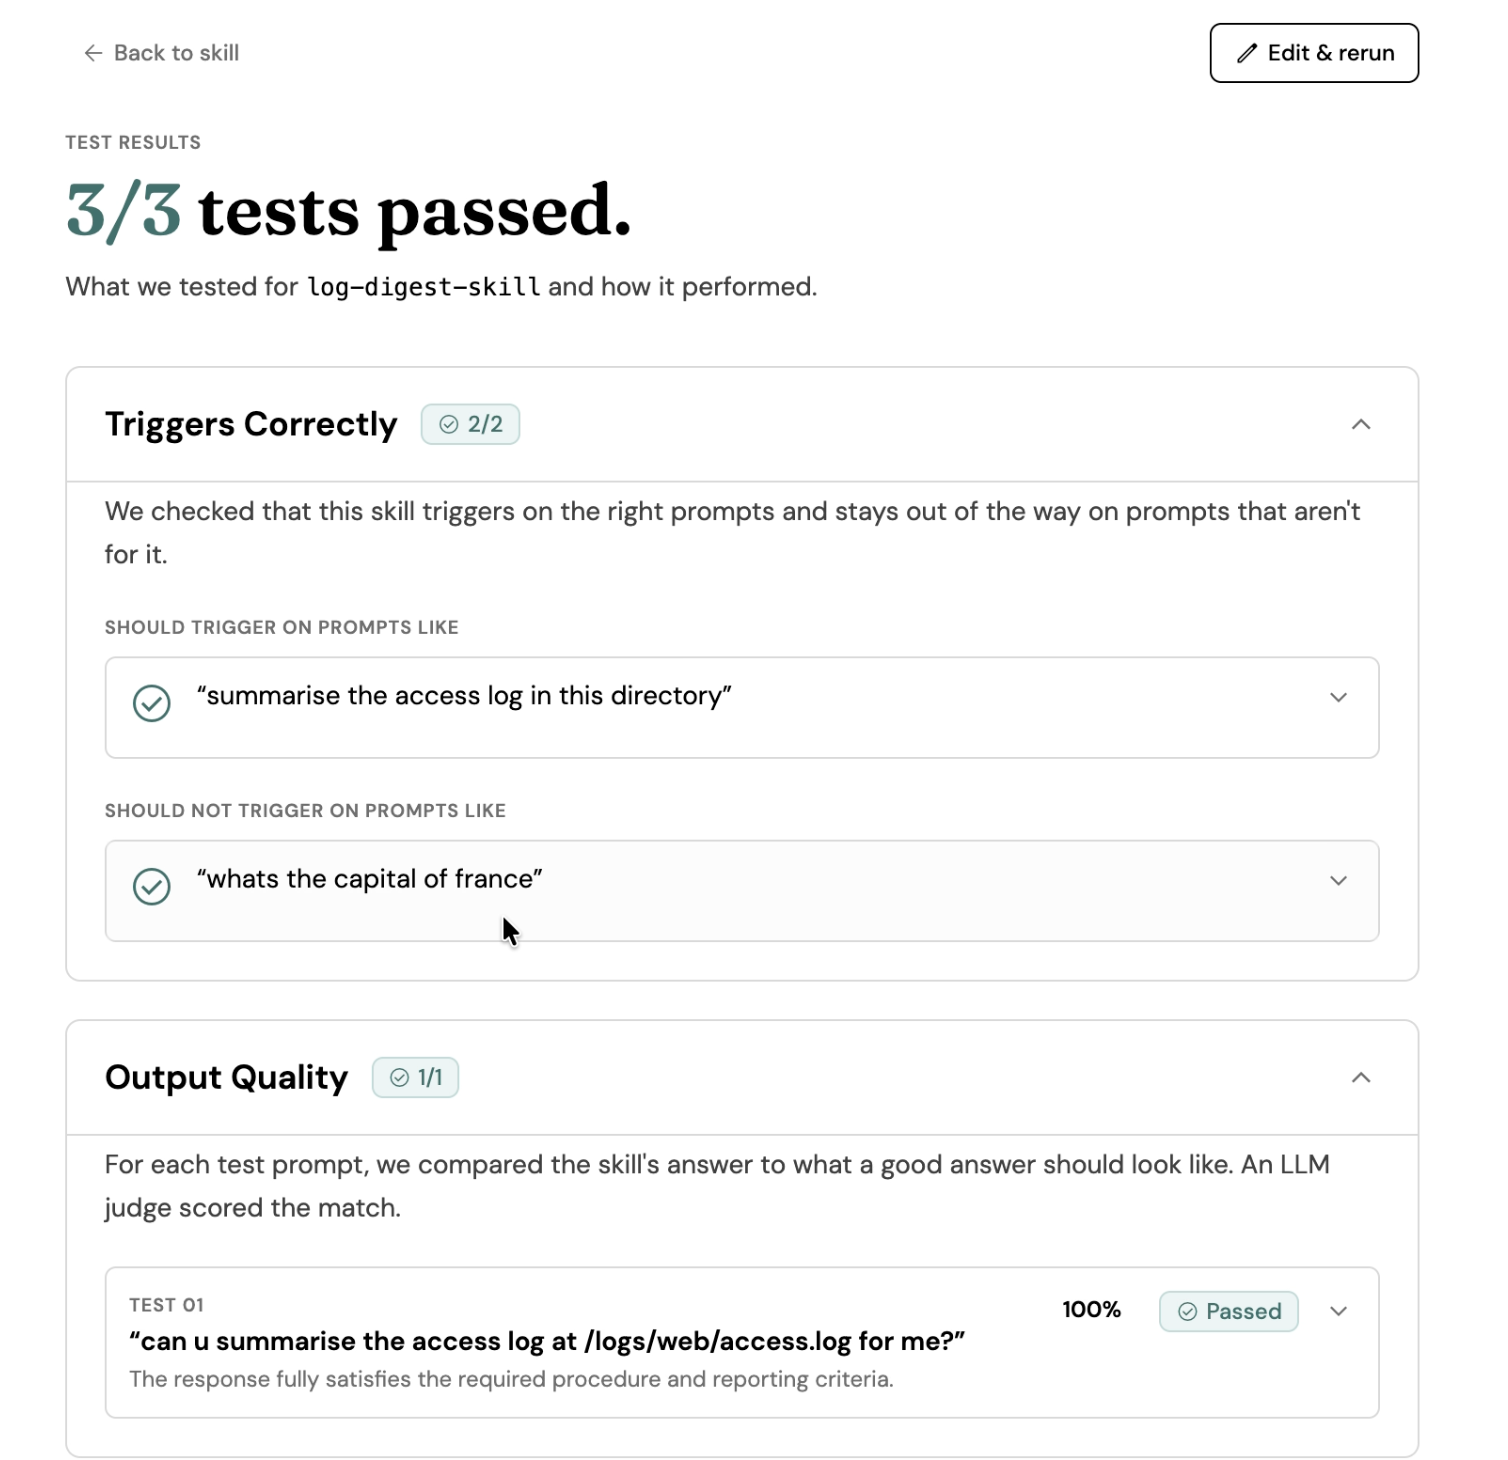
\includegraphics[width=0.62\linewidth]{figures/mk-evals-ui-10.png}
    \caption{The consolidated test-results page, summarising both dimensions for a reviewer: the headline verdict, the invocation prompts and their polarity, and the per-test quality scores with the judge's justification.}
    \label{fig:ui-results-page}
  \end{figure}
\end{enumerate}

\section{The man.evals library and command line}

\texttt{man.evals} packages the evaluation engine as a pip-installable Python library with no server, database, or web-framework dependencies, together with a thin command-line wrapper. It exists because of the two demands that came back from the Phase 2 deployment. The first is workflow-shaped: authors iterate on skills in a terminal, and the natural loop is to edit SKILL.md, run the tests, read the result, and edit again, the way a software engineer runs unit tests while editing code. Reaching a browser and a deployed server in the middle of that loop breaks it. The second demand is capability-shaped: some users want to run the agent with real tools and evaluate what it actually did, which the platform cannot offer and only the library provides. The library and the platform share one engine, and this sharing is the load-bearing property: a score obtained in the terminal means the same thing as a score obtained in the browser, because the same code with the same semantics produced both.

\subsection{Entry Points of man.evals}
The library exposes a single conceptual operation through two entry points. \texttt{run\_eval} is the Python API; \texttt{arun\_eval} is its async twin for callers already inside an event loop, identical in signature except that live progress bars default off. \texttt{man-evals} is the command-line wrapper over \texttt{run\_eval}. Table 3.1 merges the two surfaces into one view: each row is a parameter, what it controls, its Python name, its CLI flag, and its default. The table itself makes the design point that matters: the CLI adds no behaviour. Every capability reachable from the shell is a direct rendering of a library argument, so nothing an author scripts in CI can behave differently from what a colleague runs in Python.